\documentclass[10.5pt,scale=1.0,t,aspectratio=169,hyperref={pdfpagelabels=false}]{beamer}


\usepackage{lipsum}
\usepackage{color}
\usepackage{amsfonts}
\usepackage{amsmath,mathtools}
\usepackage{mathrsfs}
\usepackage{array}
\usepackage{algorithm}
\usepackage{hyperref}
\usepackage[spanish,es-nodecimaldot]{babel}
\usepackage[utf8]{inputenc}
\usepackage{graphicx}
\usepackage{multicol}
\usepackage{multirow}
\usepackage{enumitem}
\usepackage[document]{ragged2e}
\usepackage[absolute,overlay]{textpos}
\textblockorigin{0mm}{0mm} 
\usefonttheme[onlymath]{serif}
\usepackage{verbatim}
\usepackage{cite}
\usepackage{multicol}
\usepackage{siunitx}




\newenvironment{conditions}[1][where:]
{#1 \begin{tabular}[t]{>{$}l<{$} @{${}={}$} l}}
	{\end{tabular}\\[\belowdisplayskip]}


\newcolumntype{L}{>{$}l<{$}} % math-mode version of "l" column type


\newcounter{saveenumi}
\newcommand{\seti}{\setcounter{saveenumi}{\value{enumi}}}
\newcommand{\conti}{\setcounter{enumi}{\value{saveenumi}}}

\setbeamertemplate{bibliography item}{\insertbiblabel}


\hypersetup{colorlinks=true,
	linkcolor=blue,
	linktoc=all,				
	citecolor=blue,
	urlcolor=red,
	pdftitle={FUNDAMENTOS DE AUTOMATIZACIÓN Y CONTROL},
	pdfauthor={Santiago Rúa Pérez},
	pdfcreator={Santiago Rúa Pérez}}


\definecolor{GreenDark}{rgb}{0.0, 0.60, 0.0}
\definecolor{RedDark}{rgb}{183, 0.0, 0.0}
\definecolor{BlueDark}{rgb}{0.0, 0.0, 167}
\definecolor{BlueLight}{rgb}{0.2, 0.451, 0.517}


\graphicspath{{imag/}}

\newcommand{\Ho}{$H_{0}$}
\newcommand{\Ha}{$H_{a}$}
\newcommand{\Nota}{{\bf Nota: }}
\newcolumntype{P}[1]{>{\centering\arraybackslash}p{#1}}
\newcolumntype{M}[1]{>{\centering\arraybackslash}m{#1}}

\newcommand{\less}{<}
\newcommand{\greater}{>}


\setlength{\parindent}{1em}
\setlength{\parskip}{.6em}
\renewcommand{\baselinestretch}{.9}

%%%%    C environment    ---------------- %%%%%%%%%%%%%%%.
\usepackage{listings}
\usepackage{xcolor}
\definecolor{mGreen}{rgb}{0,0.6,0}
\definecolor{mGray}{rgb}{0.5,0.5,0.5}
\definecolor{mPurple}{rgb}{0.58,0,0.82}
\definecolor{backgroundColour}{rgb}{0.95,0.95,0.92}

\lstdefinestyle{CStyle}{
	backgroundcolor=\color{backgroundColour},   
	commentstyle=\color{mGreen},
	keywordstyle=\color{magenta},
	numberstyle=\tiny\color{mGray},
	stringstyle=\color{mPurple},
	basicstyle=\tiny,
	breakatwhitespace=false,         
	breaklines=true,                 
	captionpos=b,                    
	keepspaces=true,                 
	numbers=left,                    
	numbersep=5pt,                  
	showspaces=false,                
	showstringspaces=false,
	showtabs=false,                  
	tabsize=2,
	language=C
}
%%--------------------------------------------------------------------------


\title{Diseño de Sistemas Embebidos}   
\author{Santiago Rúa Pérez, PhD.} 
\date{\today} 

\setlength{\TPHorizModule}{\textwidth}
\setlength{\TPVertModule}{\textwidth}

\newcommand{\btVFill}{\vskip0pt plus 1filll}


\setbeamertemplate{sidebar right}{}
\setbeamertemplate{footline}
{
	\leavevmode%
	\hbox{%
		\begin{beamercolorbox}[wd=.333333\paperwidth,ht=2.25ex,dp=1ex,center]{author in head/foot}%
			\usebeamerfont{author in head/foot}\insertshortauthor
		\end{beamercolorbox}%
		\begin{beamercolorbox}[wd=.333333\paperwidth,ht=2.25ex,dp=1ex,center]{title in head/foot}%
			\usebeamerfont{title in head/foot}\insertshorttitle
	\end{beamercolorbox}}%
	\vskip0pt%
}
\makeatother

\begin{document}
	%%%%%%%%%%%%%%%%%% FRAME %%%%%%%%%%%%%%%%%%%%%%%%%%
	\begin{frame}
		\titlepage
	\end{frame}
	%%%%%%%%%%%%%%%%% FRAME START %%%%%%%%%%%%%%%%%%%%%%%%%%
	\frame{
		%\frametitle{}
		\begin{center}
			\LARGE \textcolor{blue}{MBED}
		\end{center}
		
	}
	
	%%%%%%%%%%%%%%%%% FRAME %%%%%%%%%%%%%%%%%%%%%%%%%%

%%%%%%%%%%%%%%%%% FRAME %%%%%%%%%%%%%%%%%%%%%%%%%%
\begin{frame}
\frametitle{Panorama general}
\begin{itemize}
\item Mbed
\item Entrada y salidas digitales
\item Entradas y salidas analogas.
\item PWM
\item Comunicaciones Seriales
\item Timers e interrupciones.
\end{itemize}
\end{frame}
%%%%%%%%%%%%%%%%% FRAME %%%%%%%%%%%%%%%%%%%%%%%%%%
\begin{frame}
	\frametitle{Porque comunicaciones seriales?}
	\begin{columns}
		\column{0.7\linewidth}
		
		\begin{itemize}
			\item Sistema operativo pensado para dispositivos IoT.
			\item Es un sistema Open Source con conectividad, almacenamiento, administración de dispositivos y machine learning. 
			\item Puede programarse de forma local o en la nube.
			\item Puede ser programado completamente con RTOS y también bare metal. 
		\end{itemize}
		
		
		\column{0.3\linewidth}
		
		\begin{figure}
			\centering
			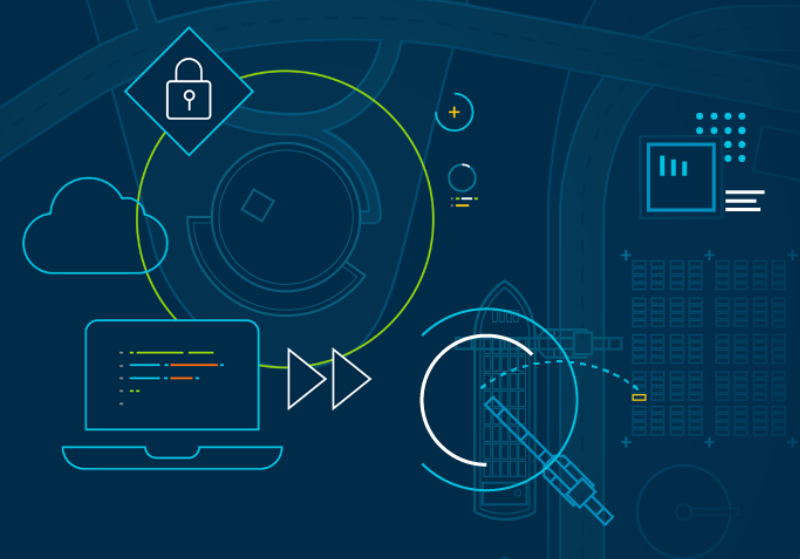
\includegraphics[scale=0.30]{01_Mbed}
		\end{figure}
	\end{columns}
\end{frame}
%%%%%%%%%%%%%%%%% FRAME %%%%%%%%%%%%%%%%%%%%%%%%%%
\begin{frame}
	\frametitle{FRDM-K64F}
	FRDM-K64F esta habilitada para trabajar con Mbed, pero se debe descargar el bootloader
	
	\begin{columns}
		\column{0.5\linewidth}
		\begin{figure}
			\centering
			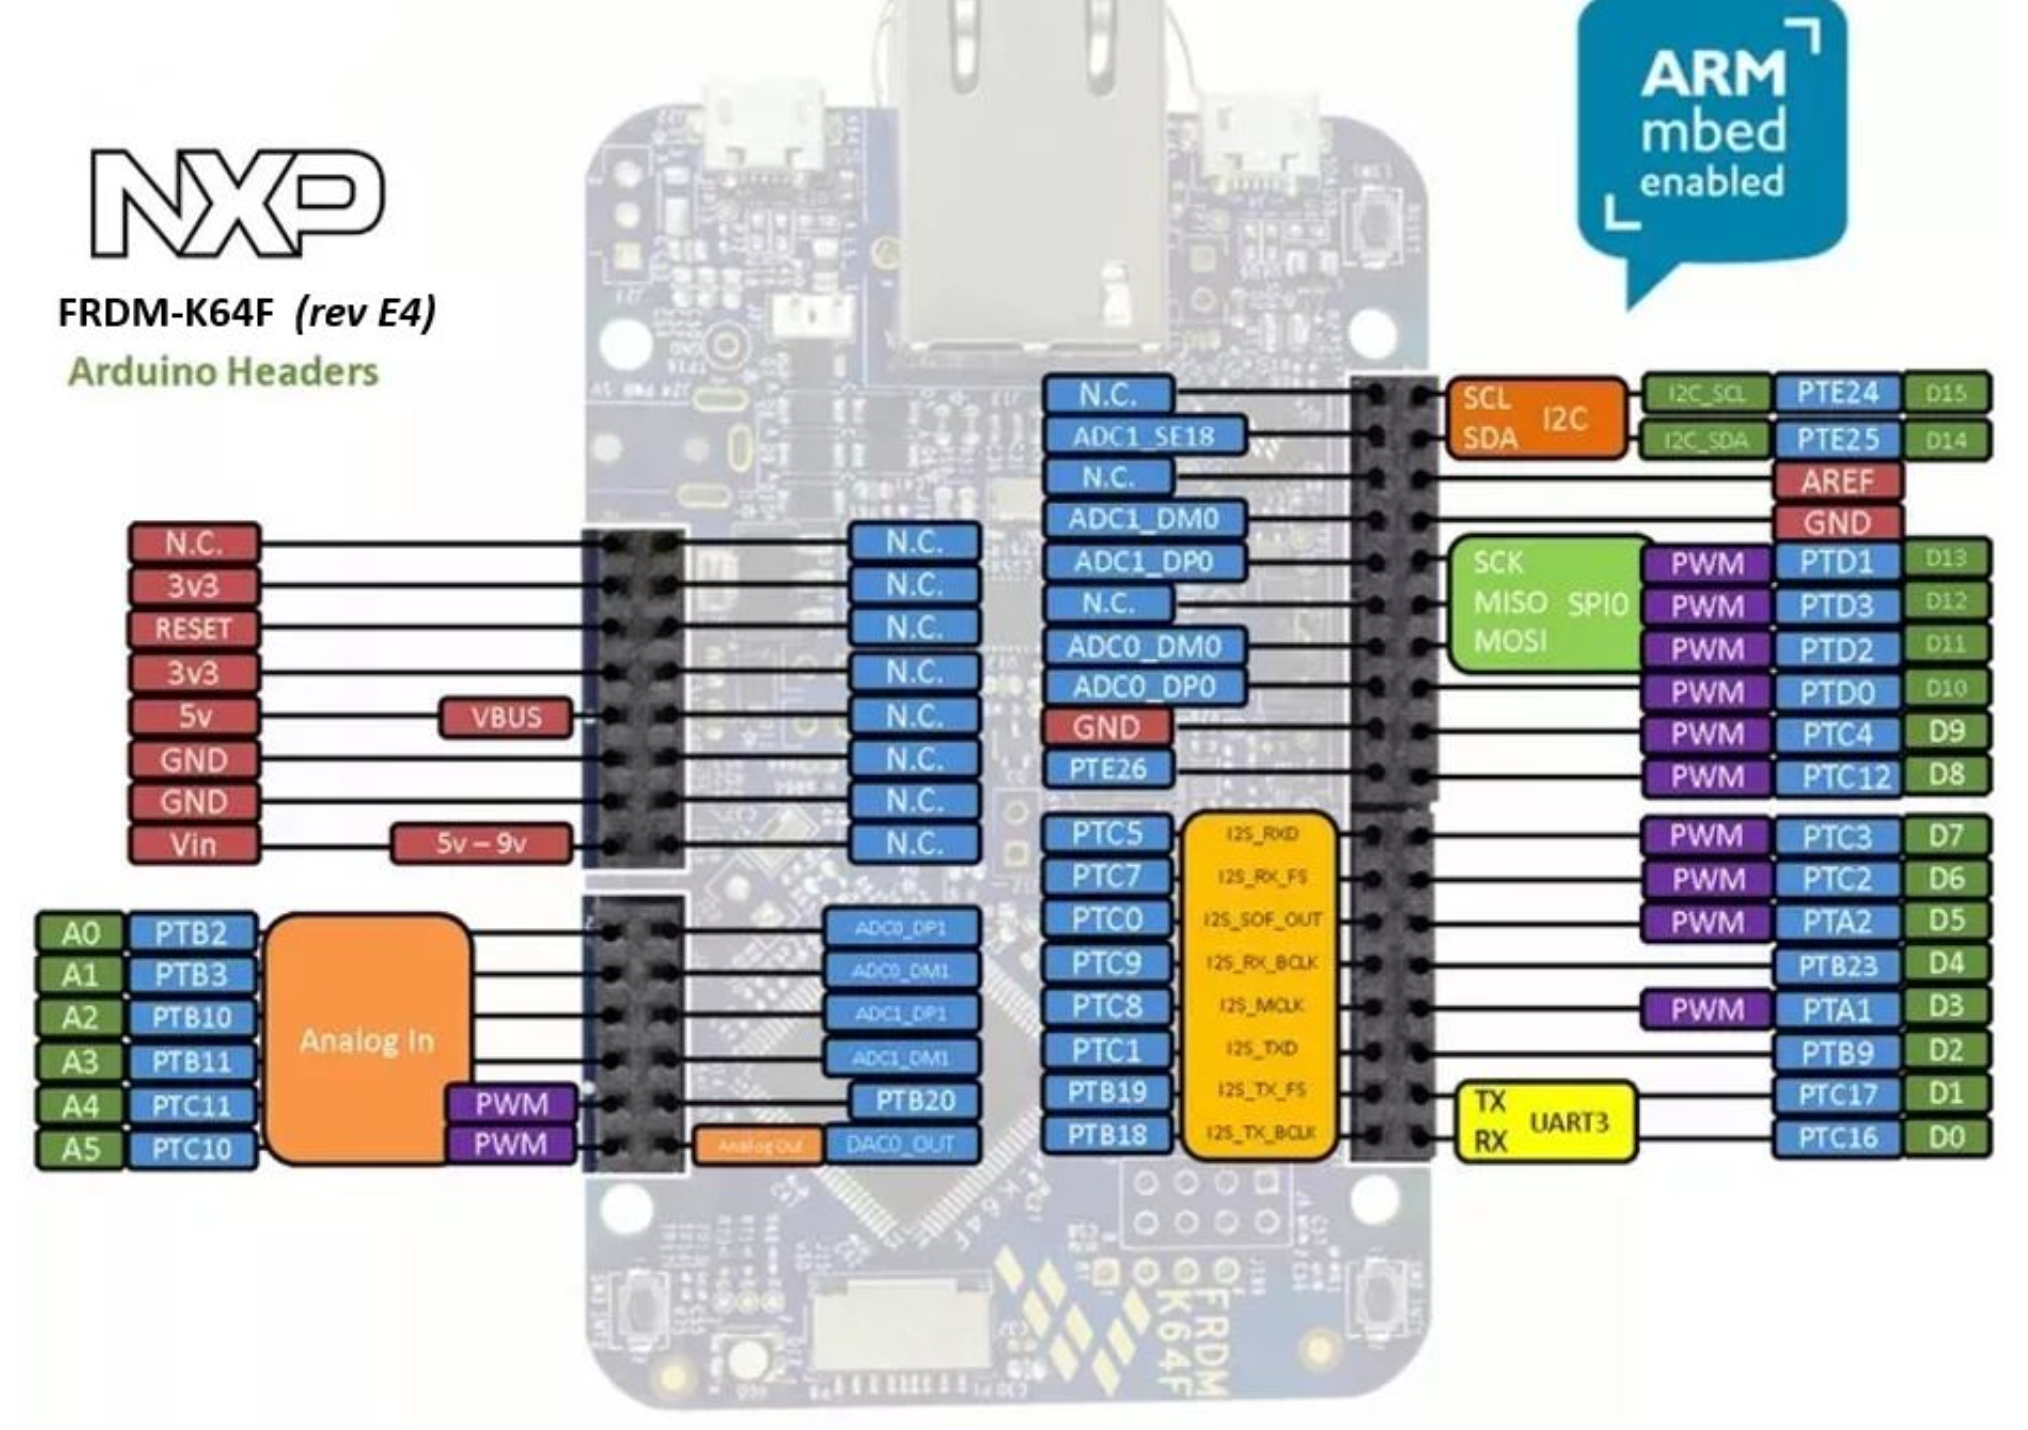
\includegraphics[scale=0.2]{02_K64F}
		\end{figure}
	
		\column{0.5\linewidth}
		\begin{itemize}
			\item \textbf{LED RGB}: LED\_RED = PTB22; LED\_GREEN = PTE26; LED\_BLUE = PTB21
			\item \textbf{Botones}: SW2 = PTC6; SW3 = PTA4  
			\item \textbf{USB pines}: USBTX = PTB17; USBRX = PTB16 
			\item \textbf{Arduino pin digitales}:  D0-D15
			\item \textbf{Análogos}: A0-A5
		\end{itemize}
	\end{columns}
	
\end{frame}
%%%%%%%%%%%%%%%%% FRAME %%%%%%%%%%%%%%%%%%%%%%%%%%
\begin{frame}
	\frametitle{Salidas Digitales con Mbed}
	En Mbed la librería de pines digitales tienen las siguientes funciones
	\begin{figure}
		\centering
		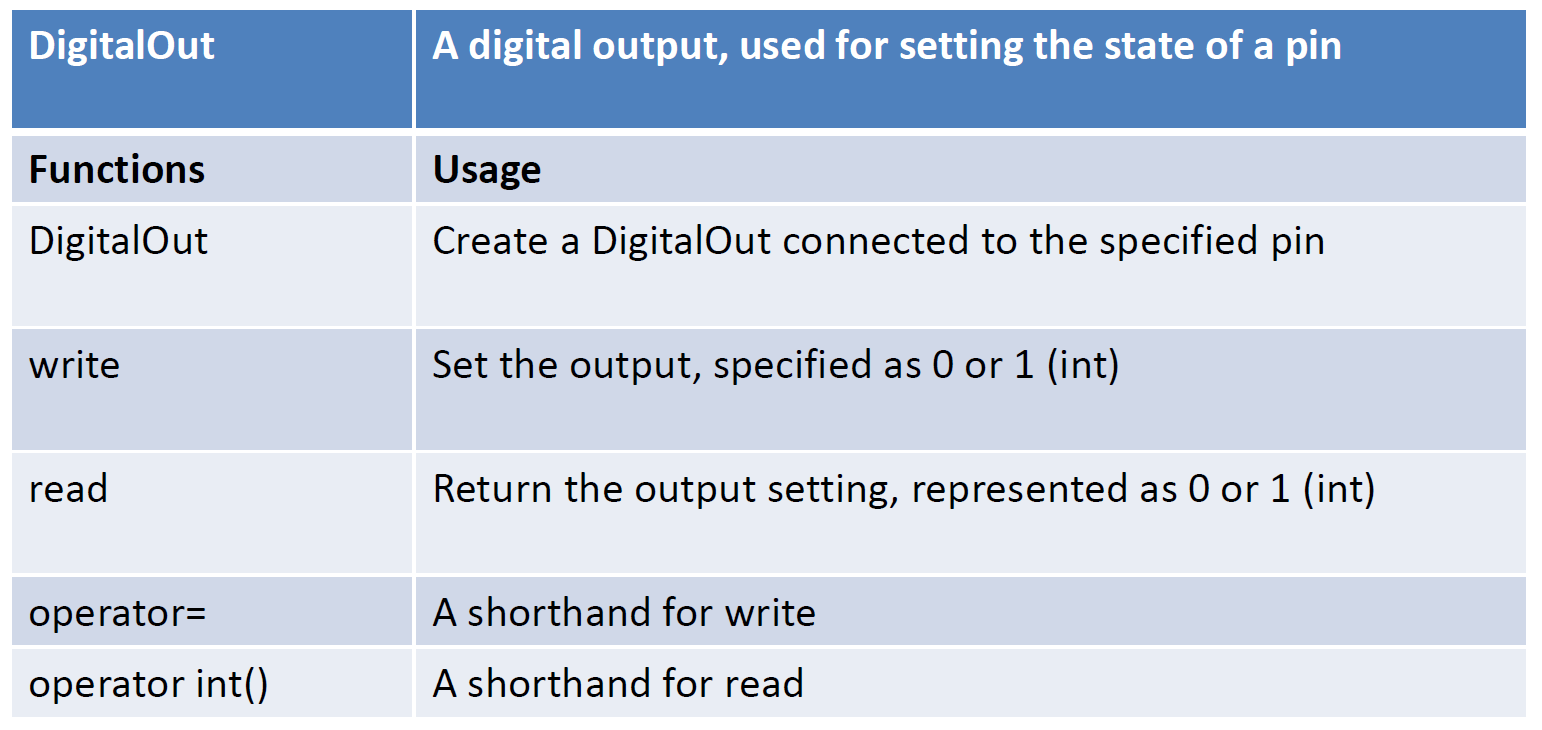
\includegraphics[scale=0.5]{03_DigitalFunctions}
	\end{figure}
\end{frame}
%%%%%%%%%%%%%%%%% FRAME %%%%%%%%%%%%%%%%%%%%%%%%%%
\begin{frame}
	\frametitle{Salidas Digitales con Mbed}
	\begin{itemize}
		\item Los pines de entrada y salida son configurados al inicio del programa
		\item Cada pin IO se le debe dar un nombre y un pin asociado, por ejemplo: DigitalOut myname1(p5);
		\item La interfaz de DigitalOut puede ser usar para poner el estado del pin y para leerlo también.
		\item Poner el pin en cero para apagarlo y en 1 para encenderlo.
		\begin{figure}
			\centering
			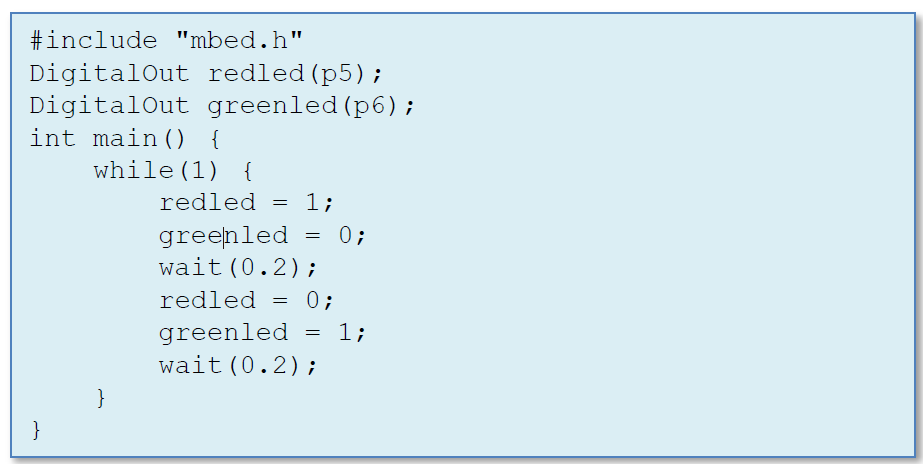
\includegraphics[scale=0.5]{04_EjemploDigitalOut}
		\end{figure}
	\end{itemize}
\end{frame}
%%%%%%%%%%%%%%%%% FRAME %%%%%%%%%%%%%%%%%%%%%%%%%%
\begin{frame}
	\frametitle{Salidas Digitales con Mbed}
	Las características principales del programa son:
	\begin{itemize}
		\item Se realiza el link a la libreria mbed.h
		\item El objeto DigitalOut se define con un nombre y se selecciona un pin (se realiza su instanciamiento) 
		\item La funcion principal del programa sigue existiendo dentro del main
		\item Se debe implementar un loop infinito while para que el programa se ejecute siempre.
		\item Basta con cambiar el valor al objeto para cambiar el estado de la salida
		\item Accedemos a capacidades de C++ para multihilos y funciones de tiempo. 
	\end{itemize}
\end{frame}
%%%%%%%%%%%%%%%%% FRAME %%%%%%%%%%%%%%%%%%%%%%%%%%
\begin{frame}
	\frametitle{Entradas Digitales con Mbed}
	\begin{itemize}
		\item Las entradas digitales son valores que pueden ser leídos.
		\item Los mismos pines digitales pueden ser configurados como entradas utilizando la misma convención pero cambiando la palabra por DigitalIn.  
		\item La interfaz digital determina el estado lógico del pin, si es cero o uno.
		\item Para cada sistema embebidos este dependerá de la alimentación del mismo. 
	\end{itemize}
\end{frame}
%%%%%%%%%%%%%%%%% FRAME %%%%%%%%%%%%%%%%%%%%%%%%%%
\begin{frame}
	\frametitle{Entradas Digitales con Mbed}
	En Mbed la librería de pines digitales tienen las siguientes funciones
	\begin{figure}
		\centering
		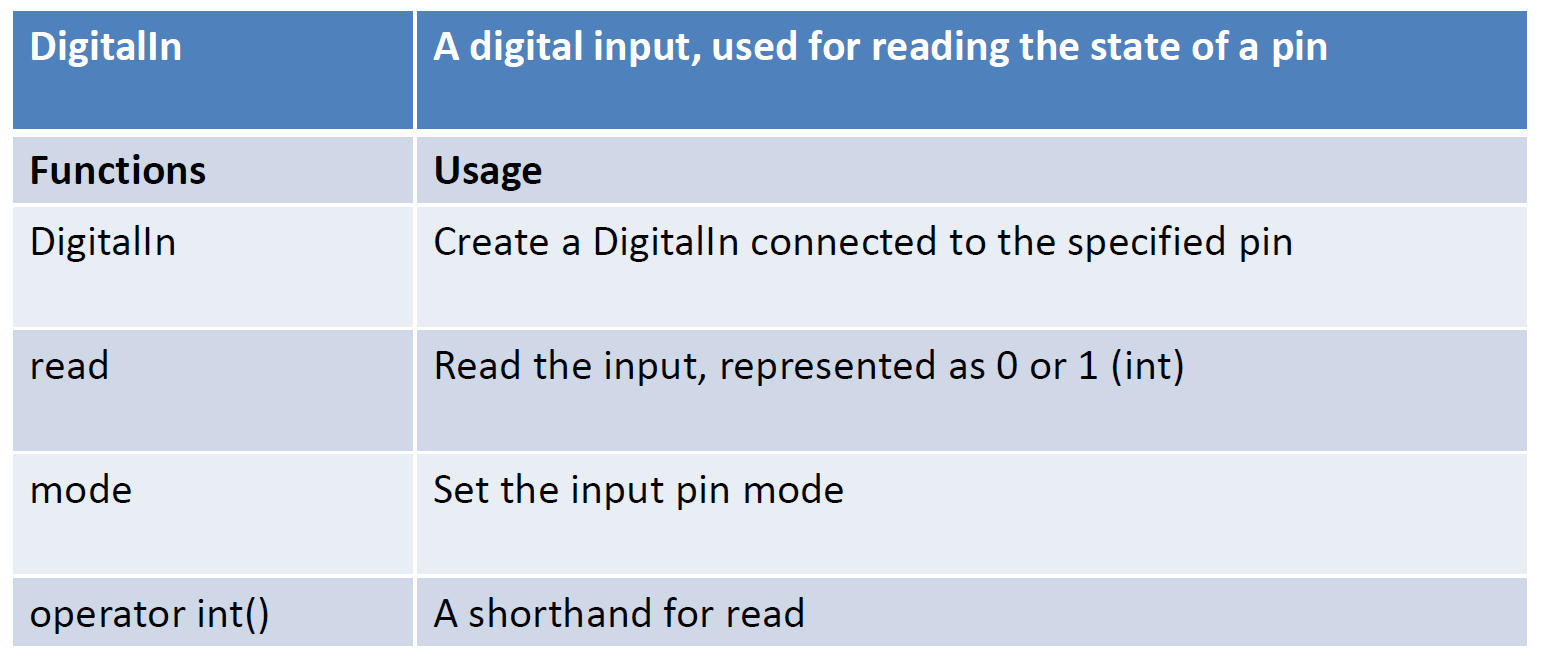
\includegraphics[scale=0.5]{05_DigitalInFunctions}
	\end{figure}
\end{frame}
%%%%%%%%%%%%%%%%% FRAME %%%%%%%%%%%%%%%%%%%%%%%%%%
\begin{frame}
	\frametitle{Entradas Digitales con Mbed - Ejemplo}
	\begin{columns}
		\column{0.5\linewidth}
		\begin{itemize}
			\item Cree un programa en donde si el pulsador esta presionado haga una secuencia de led diferente a cuando no esta pulsado.
			\item Si el pulsador es cero entonces se realiza la secuencia de verde, sino se realiza la secuencia de rojo. 
			\item \textbf{Tarea}: cree una senal digital de 1000Hz que pueda ser leida con osciloscopio
		\end{itemize}
		 
		
		\column{0.5\linewidth}
		\begin{figure}
			\centering
			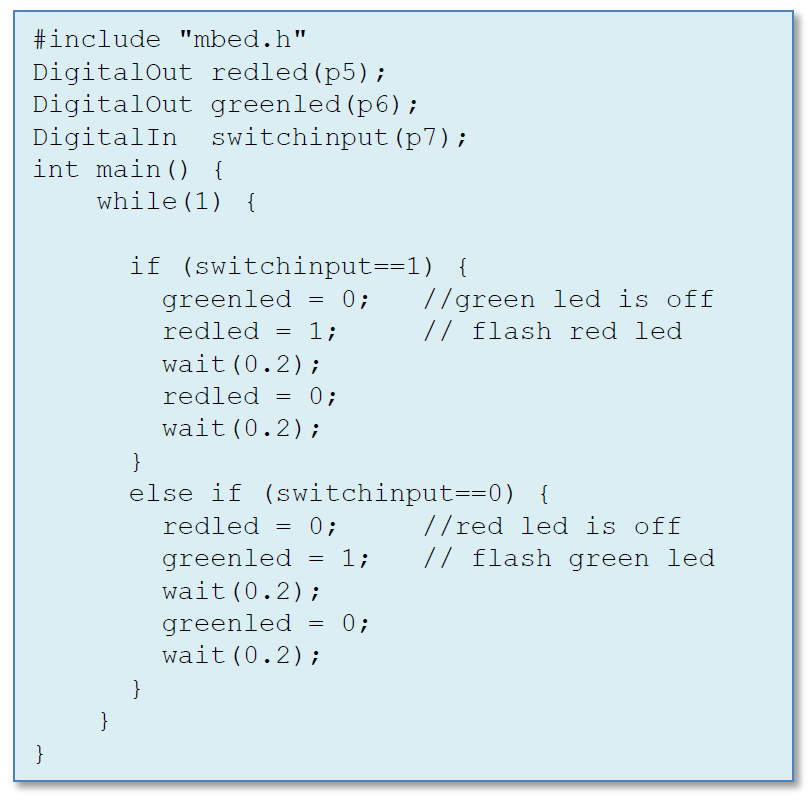
\includegraphics[scale=0.35]{06_EjemploIn}
		\end{figure}
	\end{columns}
\end{frame}
%%%%%%%%%%%%%%%%% FRAME %%%%%%%%%%%%%%%%%%%%%%%%%%
\begin{frame}
	\frametitle{Y los demás periféricos ...}
	Que falta por mirar? Se puede ver de nuevo todo el curso con los módulos que ya se trabajaron y siguiendo la filosofía de Mbed
	\begin{itemize}
		\item \href{https://os.mbed.com/docs/mbed-os/v6.15/apis/analogout.html}{Salidas} y \href{https://os.mbed.com/docs/mbed-os/v6.15/apis/i-o-apis.html}{entradas} análogas.
		\item \href{https://os.mbed.com/docs/mbed-os/v6.15/apis/pwmout.html}{PWM}
		\item Comunicaciones seriales: \href{https://os.mbed.com/docs/mbed-os/v6.15/apis/spi.html}{SPI}, \href{https://os.mbed.com/docs/mbed-os/v6.15/apis/serial-uart-apis.html}{UART}, \href{https://os.mbed.com/docs/mbed-os/v6.15/apis/i2c.html}{I2C}
		\item \href{https://os.mbed.com/docs/mbed-os/v6.15/apis/timer.html}{Timers} e \href{https://os.mbed.com/docs/mbed-os/v6.15/apis/interruptin.html}{interrupciones}
		\item Otras clases interesantes:
		\begin{itemize}
			\item Manejo de \href{https://os.mbed.com/docs/mbed-os/v6.15/apis/busout.html}{buses}
			\item Protocolo \href{https://os.mbed.com/docs/mbed-os/v6.15/apis/other-driver-apis.html}{CAN}
		\end{itemize}
	\end{itemize}
\end{frame}
%%%%%%%%%%%%%%%%% FRAME %%%%%%%%%%%%%%%%%%%%%%%%%%
\frame{
\begin{center}
	\LARGE \textcolor{blue}{MBED}
\end{center}

\begin{center}
	\LARGE \textcolor{blue}{GRACIAS}
\end{center}
}

%%%%%%%%%%%%%%%%%%%%%%%%%%%%%%%%%%%%%%%%%%%%%%%%%%%%%%%%%%%%%%%%%%%%%%%%%%%%%%%%%%%%%%%%%%%%%%%%%%%%%%%%%%%%%



\end{document}

